\chapter{Состояния, измерения и комплексные векторные пространства}

\lectureoverview{Квантовая механика начинается с изменения того, что мы понимаем под состоянием. Сначала мы выделим классическую схему состояний и детерминированного обновления, а затем с помощью спинового эксперимента с двумя исходами покажем её несостоятельность. Математическим ответом служит комплексное векторное пространство, снабжённое дуальными векторами, скалярным произведением, нормой и отношением ортогональности.}

\section{Классическая схема: состояние и обновление}

Начнём с замкнутой системы, по крайней мере временно изолированной от всего остального. Слово \emph{система} здесь является первичным: оно означает объект, историю которого мы хотим предсказать. \emph{Состояние} — это всё, что необходимо знать в один момент времени, чтобы сделать такое предсказание. Классическая механика задаёт закон, который переводит одно состояние в следующее.

Для самой простой абстрактной монеты,
\begin{equation}
  \mathcal S_{\mathrm{coin}}=\{H,T\}.
\end{equation}
Один из возможных законов утверждает, что ничего не происходит:
\begin{equation}
  H\longmapsto H,
  \qquad
  T\longmapsto T.
\end{equation}
Другой закон чередует два состояния:
\begin{equation}
  H\longmapsto T,
  \qquad
  T\longmapsto H.
\end{equation}
Эти примеры элементарны, но они выявляют устройство классической теории:
\begin{equation}
  s(t)\longmapsto s(t+\Delta t).
\end{equation}
Как только известно \(s(t)\), обновление детерминировано.

Та же схема сохраняется и тогда, когда пространство состояний непрерывно. Частица, движущаяся по прямой, требует задания как положения, так и импульса,
\begin{equation}
  s=(q,p),
\end{equation}
поэтому её пространством состояний служит фазовая плоскость. Число возможных состояний стало бесконечным, а уравнения можно записывать на элегантном языке лагранжианов, гамильтонианов и скобок Пуассона, но лежащая в основе идея не изменилась. Состояние в один момент времени содержит всё, что нужно для предсказания состояния в другой.

\section{Абстракция прежде наглядности}

Классическое движение сравнительно легко представить, потому что его понятия взяты из повседневного опыта. Это преимущество исчезает, когда существенные объекты слишком малы, скорости слишком велики или размерность пространства состояний слишком высока. Никто не визуализирует в буквальном смысле движение электрона, четырёхмерное пространство-время или десятимерное пространство. Это не недостаток, свойственный только начинающим. Зрительная интуиция человека сформировалась для повседневного трёхмерного мира.

Даже случаи, которые кажутся более простыми, обнаруживают это ограничение. То, что мы называем изображением двумерного искривлённого пространства, обычно представляет собой поверхность, вложенную в трёхмерное пространство. Одномерную прямую изображают как черту на плоскости. При таком изображении незаметно привносится объемлющее пространство, в котором наша зрительная система умеет работать.

Выход не в том, чтобы навязывать незнакомой физике классическую картину. Нужно освоить абстрактную структуру и позволить новой интуиции вырасти из правильных операций. Трёхмерные координаты \((x,y,z)\) превращаются в четырёхмерные координаты \((x,y,z,w)\) посредством добавления одного символа и расширения правил, а не благодаря приобретению нового органа зрения. Квантовая механика требует той же дисциплины. Обращение с ней как со странной механической моделью маленьких классических объектов будет раз за разом приводить к неверному ответу.

\begin{remark}
Математическая интуиция всё же развивается. Просто она не тождественна зрительному восприятию волны в океане или стрелки в обычном пространстве. Алгебра становится привычной, потому что её соотношения используются последовательно.
\end{remark}

\section{Классические пространства состояний и классическая логика}

Для классической системы пространство состояний — это множество. Абстрактный игральный кубик имеет
\begin{equation}
  \mathcal S_{\mathrm{die}}=\{1,2,3,4,5,6\}.
\end{equation}
Реальный кубик имеет континуально много ориентаций, но идеализированный кубик, рассматриваемый здесь, имеет только эти шесть меток. Частица на прямой имеет континуально бесконечное множество
\begin{equation}
  \mathcal S_{\mathrm{particle}}
  =
  \{(q,p)\mid q,p\in\mathbb R\}.
\end{equation}
Конечно оно или бесконечно, каждое классическое пространство состояний есть совокупность взаимно различных возможностей.

Высказывание о системе выделяет подмножество этих возможностей. Для кубика положим
\begin{align}
  P_{\mathrm{odd}}&=\{1,3,5\},\\
  P_{\leq 3}&=\{1,2,3\}.
\end{align}
Утверждение \emph{нечётно и не больше трёх} соответствует их пересечению:
\begin{equation}
  P_{\mathrm{odd}}\cap P_{\leq 3}=\{1,3\}.
\end{equation}
Утверждение \emph{нечётно или не больше трёх}, где «или» понимается как неисключающее, соответствует их объединению:
\begin{equation}
  P_{\mathrm{odd}}\cup P_{\leq 3}
  =
  \{1,2,3,5\}.
\end{equation}
Таким образом, в классическом случае конъюнкция и дизъюнкция имеют теоретико-множественную форму
\begin{equation}
  P\wedge Q\longleftrightarrow P\cap Q,
  \qquad
  P\vee Q\longleftrightarrow P\cup Q.
\end{equation}
Если подмножества не пересекаются, ни одно состояние не делает оба высказывания истинными.

Эта логика связана с классическим пониманием состояния. В квантовой механике множество классических альтернатив заменяется другим математическим объектом: векторным пространством. Лишь в подходящем классическом пределе описание в терминах векторного пространства ведёт себя приближённо как множество взаимоисключающих конфигураций. Прежде чем построить это пространство, нам нужен эксперимент, делающий такую замену неизбежной.

\section{Простейшая квантовая система}

Квантовым аналогом абстрактной монеты служит система с двумя исходами, называемая \emph{кубитом}. Её измеряемые альтернативы можно сначала обозначить как орёл и решка, но числовая метка полезнее:
\begin{equation}
  \sigma\in\{+1,-1\}.
\end{equation}
Далее будут параллельно использоваться три обозначения:
\begin{equation}
  H\longleftrightarrow \sigma=+1\longleftrightarrow\uparrow,
  \qquad
  T\longleftrightarrow \sigma=-1\longleftrightarrow\downarrow.
\end{equation}
Поначалу стрелки — лишь обозначения. Никакой обычный геометрический вектор пока не предполагается.

\begin{figure}[htbp]
  \centering
  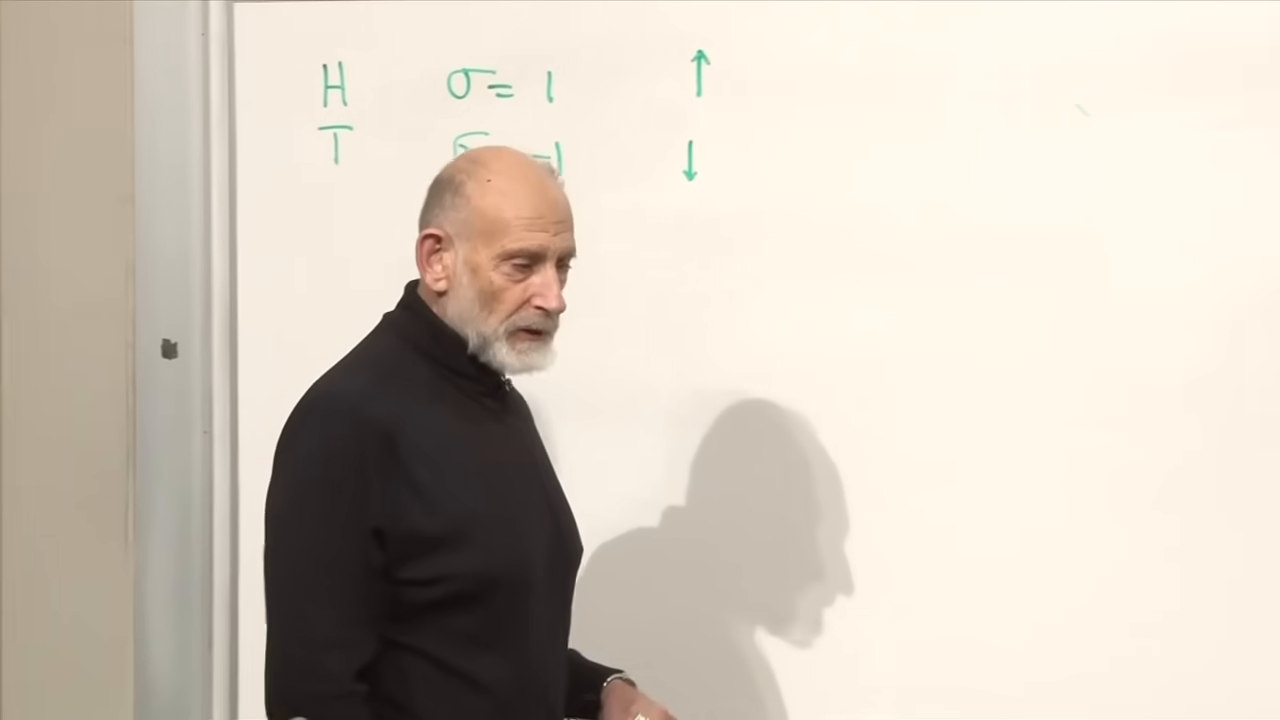
\includegraphics[width=0.78\textwidth]{lecture_01_figure_02.png}
  \caption{На доске вводятся эквивалентные обозначения \(H/T\), \(\sigma=\pm1\) и стрелки вверх/вниз. Стрелки здесь изначально служат обозначениями, а не классической моделью.}
  \lectureframe{00:22:44}
\end{figure}

\begin{classroomqa}
\audiencequestion{Какое отношение орёл и решка имеют к физической системе?}
\lecturerresponse{Никакого, кроме того, что они дают два знакомых названия. У кубита для этого измерения есть два возможных исхода; орёл и решка служат лишь условными обозначениями. Метки \(\pm1\) выбраны потому, что они могут входить в уравнения.}
\end{classroomqa}

\subsection{Аппарат как чёрный ящик}

Эксперимент требует второй системы — аппарата \(A\). Пока что это абстрактный чёрный ящик с тремя свойствами:
\begin{enumerate}
  \item он имеет пространственную ориентацию, отмеченную как \emph{этой стороной вверх};
  \item у него есть датчик, способный взаимодействовать с кубитом;
  \item у него есть индикатор, который сначала пуст, а затем показывает \(+1\) или \(-1\).
\end{enumerate}
Устройство детектора намеренно оставлено без подробностей. Хороший детектор определяется операционально надёжной связью между системой и записью о ней. Наблюдателю не обязательно смотреть в момент взаимодействия; аппарат может зарегистрировать результат, а прочитать его можно позже.

Предположим, что индикатор показывает \(+1\). Вернём аппарат в исходное пустое состояние и немедленно повторим то же измерение, прежде чем успеет подействовать какая-либо самостоятельная эволюция. Надёжный детектор снова показывает \(+1\). Если первый результат равен \(-1\), то и при немедленных повторениях он так же продолжает показывать \(-1\):
\begin{equation}
\begin{aligned}
  +1&\longrightarrow +1\longrightarrow +1\longrightarrow\cdots,\\
  -1&\longrightarrow -1\longrightarrow -1\longrightarrow\cdots.
\end{aligned}
\end{equation}
Поэтому первое измерение можно рассматривать как \emph{подготовку}. Оно оставляет кубит в состоянии, для которого немедленное повторение того же измерения имеет определённый результат.

Эта повторяемость — не факультативный философский комментарий. Без неё не было бы операционального способа подтвердить измерение. Неисправный прибор может не воспроизводить свой результат, но тогда он не осуществляет то идеальное измерение, которое здесь определяется.

\begin{classroomqa}
\audiencequestion{Это уже коллапс волновой функции?}
\lecturerresponse{Этот язык можно ввести позже. На данном этапе достаточно операционального утверждения: измерение даёт результат и подготавливает состояние, в котором то же самое немедленное измерение воспроизводит этот результат. Назвать процесс — ещё не значит его объяснить.}
\end{classroomqa}

\section{Ориентация и несостоятельность классической стрелки}

Подготовьте кубит так, чтобы аппарат в вертикальном положении показывал \(+1\). Поверните аппарат на \(180^\circ\) и повторите измерение. Теперь результат равен \(-1\). Повторные измерения с перевёрнутым аппаратом подтверждают \(-1\), тогда как возвращение аппарата в вертикальное положение снова даёт \(+1\).

Этот результат обнаруживает подлинную направленность. Обозначения вверх/вниз не вполне произвольны: переворот детектора меняет знак на противоположный. Возникает соблазн заключить, что кубит — это просто маленький вектор и что детектор измеряет компоненту этого вектора вдоль собственной оси. Этому соблазну нужно не доверять, а проверить его.

\begin{figure}[htbp]
  \centering
  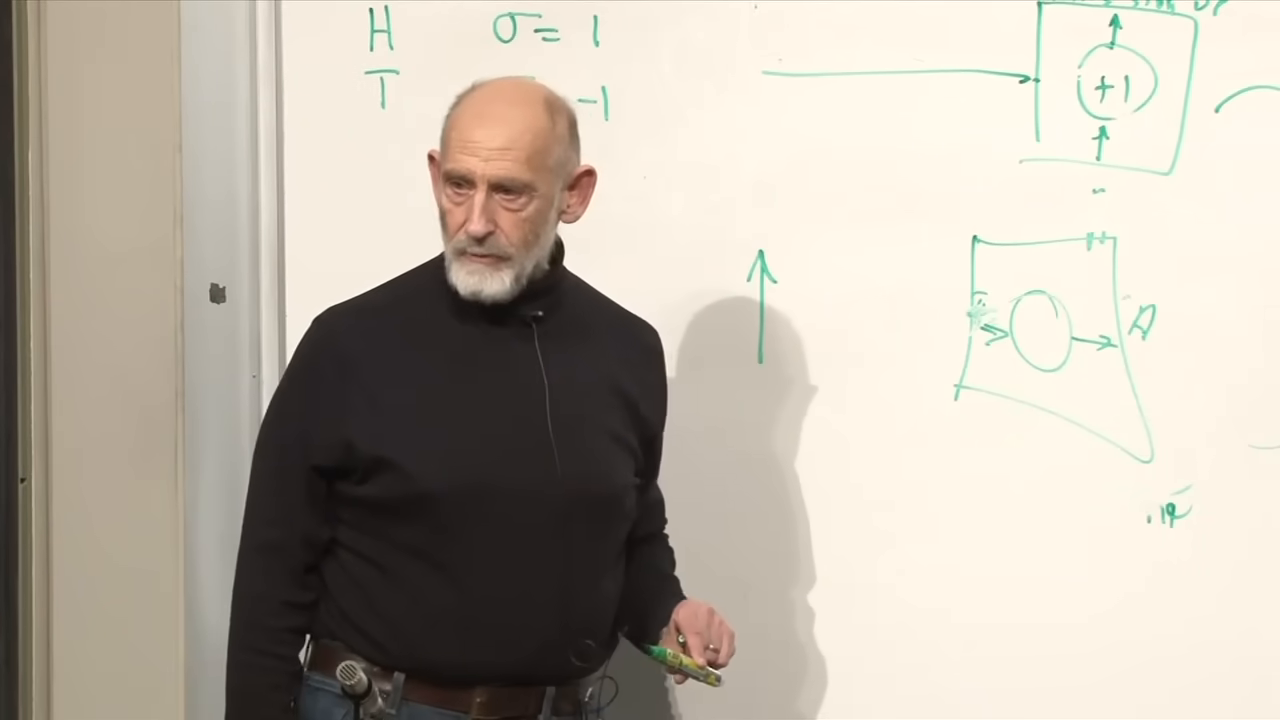
\includegraphics[width=0.82\textwidth]{lecture_01_figure_03.png}
  \caption{Подготовка вверх и по-разному ориентированные анализаторы на доске. Позже в аудитории исправили направление одной меловой стрелки; в рассуждении важна только ось анализатора.}
  \lectureframe{00:36:21}
\end{figure}

\subsection{Боковое измерение}

Поверните детектор на \(90^\circ\). Если бы подготовленный кубит был обычной стрелкой, направленной вверх, его компонента вдоль горизонтальной оси детектора была бы равна нулю:
\begin{equation}
  \hat{\mathbf x}\cdot\hat{\mathbf z}=0.
\end{equation}
Квантовый аппарат никогда не показывает нуль. Каждый отдельный опыт даёт либо \(+1\), либо \(-1\).

\begin{figure}[htbp]
  \centering
  \resizebox{\linewidth}{!}{%
  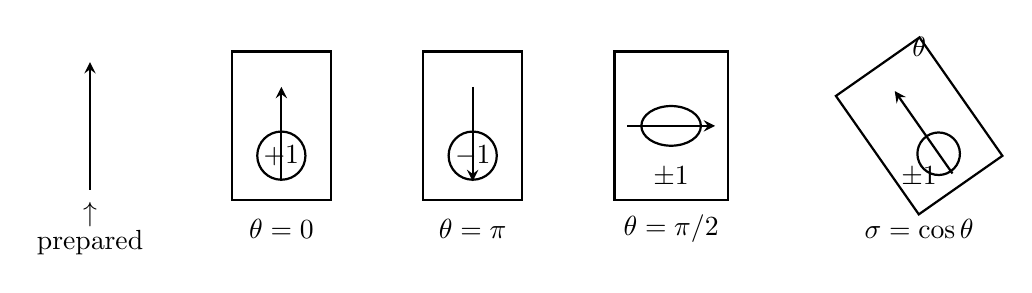
\begin{tikzpicture}[>=stealth,thick,scale=0.90]
    \draw[->] (0,0)--(0,1.8);
    \node at (0,-0.35) {\(\uparrow\)};
    \node at (0,-0.75) {prepared};

    \draw (2.0,-0.15) rectangle (3.4,1.95);
    \draw (2.7,0.48) circle (0.34);
    \draw[->] (2.7,0.12)--(2.7,1.45);
    \node at (2.7,0.48) {\(+1\)};
    \node at (2.7,-0.55) {\(\theta=0\)};

    \draw (4.7,-0.15) rectangle (6.1,1.95);
    \draw (5.4,0.48) circle (0.34);
    \draw[->] (5.4,1.45)--(5.4,0.12);
    \node at (5.4,0.48) {\(-1\)};
    \node at (5.4,-0.55) {\(\theta=\pi\)};

    \draw (7.4,-0.15) rectangle (9.0,1.95);
    \draw (8.2,0.90) ellipse (0.42 and 0.28);
    \draw[->] (7.58,0.90)--(8.82,0.90);
    \node at (8.2,0.18) {\(\pm1\)};
    \node at (8.2,-0.55) {\(\theta=\pi/2\)};

    \begin{scope}[shift={(11.7,0.90)},rotate=35]
      \draw (-0.72,-1.02) rectangle (0.72,1.02);
      \draw (0,-0.48) circle (0.30);
      \draw[->] (0,-0.82)--(0,0.60);
    \end{scope}
    \node at (11.7,0.18) {\(\pm1\)};
    \node at (11.7,-0.55) {\(\expect{\sigma}=\cos\theta\)};
    \node at (11.7,2.02) {\(\theta\)};
  \end{tikzpicture}
  }%
  \caption{Реконструкция последовательности анализаторов. Поворот изменяет статистику, но никогда не множество индивидуальных исходов.}
\end{figure}

Подготовьте большой набор кубитов с помощью вертикального анализатора, оставляя те, для которых результат равен \(+1\). Измерьте каждый сохранённый кубит один раз горизонтальным анализатором. В половине испытаний получается \(+1\), в половине — \(-1\), и среднее по ансамблю равно нулю:
\begin{equation}
  \expect{\sigma}_{\pi/2}=0.
\end{equation}
Среднее похоже на исчезающую горизонтальную компоненту классического указателя, но отдельные результаты — нет. Классическое значение \(0\) заменено статистическим балансом между двумя дискретными исходами.

\begin{classroomqa}
\audiencequestion{Что происходит, если после горизонтального измерения тот же кубит сохраняют, а не отбрасывают?}
\lecturerresponse{Предположим, что его первый горизонтальный результат — \(+1\). Если повторять горизонтальное измерение на том же кубите, снова и снова получается \(+1\). Первое горизонтальное измерение подготовило его относительно горизонтальной оси. Чтобы получить статистику пятьдесят на пятьдесят, нужно повторить весь эксперимент по подготовке и измерению на многих кубитах, а не многократно подтверждать один и тот же результат.}
\end{classroomqa}

\subsection{Несовместимые подготовки}

Порядок осей важен. Подготовьте \(+1\) вдоль вертикальной оси, затем измерьте по горизонтали. Первый горизонтальный результат случаен. После того как уже получен некоторый горизонтальный результат, немедленные повторения горизонтального измерения дают определённый ответ. Теперь поверните детектор обратно к вертикальной оси. Вертикальный результат снова случаен.

В обозначениях, где \(M_z\) и \(M_x\) обозначают измерения вдоль двух осей,
\begin{equation}
\begin{aligned}
  M_z&:+1,\\
  M_x&:\pm1,\\
  M_x&:\text{same result},\\
  M_z&:\pm1.
\end{aligned}
\end{equation}
Промежуточное измерение по \(x\) не просто выявило горизонтальную компоненту, сохранив исходное состояние с определённостью по вертикали. Оно подготовило новое состояние, и исходная вертикальная определённость исчезла.

\begin{classroomqa}
\audiencequestion{Помнит ли детектор первый ответ? Как он может знать, подан ли тот же кубит или новый?}
\lecturerresponse{Повторяемость — свойство измеряемого кубита, а не скрытое сравнение по памяти, которое выполняет детектор. После измерения кубит находится в состоянии, дающем тот же ответ на то же самое немедленное измерение. Если предъявить кубит, подготовленный иначе, результат зависит от этой подготовки. Отслеживание того, какая именно физическая система измеряется, — это обычный лабораторный учёт.}
\end{classroomqa}

\begin{classroomqa}
\audiencequestion{Значит, сам акт наблюдения подготавливает данный кубит?}
\lecturerresponse{Да. Как только это измерение подготовило кубит, то же самое измерение даёт тот же ответ, пока не вмешается какая-либо другая эволюция или несовместимое измерение.}
\end{classroomqa}

\section{Произвольно повёрнутый анализатор}

Пусть ось детектора образует угол \(\theta\) с осью, вдоль которой был подготовлен ансамбль. В каждом испытании по-прежнему получается
\begin{equation}
  \sigma=\pm1.
\end{equation}
Относительные частоты зависят от угла так, что среднее равно
\begin{equation}
  \expect{\sigma}_{\theta}=\cos\theta.
  \label{eq:qml1-cosine-mean}
\end{equation}
Предельные случаи таковы:
\begin{align}
  \expect{\sigma}_{0}&=+1,\\
  \expect{\sigma}_{\pi/2}&=0,\\
  \expect{\sigma}_{\pi}&=-1.
\end{align}
Вблизи \(\theta=0\) большинство исходов — \(+1\), изредка встречается \(-1\). Вблизи \(\theta=\pi\) большинство исходов — \(-1\), изредка встречается \(+1\).

\begin{figure}[htbp]
  \centering
  \includegraphics[width=0.82\textwidth]{lecture_01_figure_04.png}
  \caption{Фактическая запись на доске для эксперимента с произвольным углом: вертикально подготовленный ансамбль входит в анализатор, наклонённый на \(\theta\).}
  \lectureframe{00:48:55}
\end{figure}

Плавно меняющаяся вектороподобная величина — это среднее по ансамблю, а не отдельный результат. Если \(p_+(\theta)\) и \(p_-(\theta)\) — две вероятности, то
\begin{equation}
  p_+ + p_-=1,
  \qquad
  p_+-p_-=\cos\theta.
\end{equation}
Следовательно,
\begin{equation}
\begin{aligned}
  p_+(\theta)&=\frac{1+\cos\theta}{2}
  =\cos^2\frac{\theta}{2},\\
  p_-(\theta)&=\frac{1-\cos\theta}{2}
  =\sin^2\frac{\theta}{2}.
\end{aligned}
  \label{eq:qml1-half-angle-probabilities}
\end{equation}
\editorialnote{В лекции указаны два исхода и их среднее \(\cos\theta\). Уравнение~\eqref{eq:qml1-half-angle-probabilities} является непосредственным алгебраическим следствием этих утверждений и явно записывает подразумеваемый закон частот.}

\begin{classroomqa}
\audiencequestion{Показывало бы ли неподготовленное множество кубитов то же среднее \(\cos\theta\)?}
\lecturerresponse{В неполяризованном ансамбле не выделено никакого направления, поэтому его среднее равно нулю. Зависимость от \(\theta\) относится к ансамблю, который сначала был подготовлен вдоль определённой оси.}
\end{classroomqa}

\begin{classroomqa}
\audiencequestion{Почему необходим целый ансамбль, если у кубита нет промежуточной динамики?}
\lecturerresponse{Первое измерение наклонённым анализатором на одном кубите даёт один случайный исход. Каждое немедленное повторение на том же кубите лишь подтверждает этот исход. Независимые испытания требуют одинаково подготовленных кубитов, каждый из которых измеряется один раз наклонённым анализатором.}
\end{classroomqa}

\begin{classroomqa}
\audiencequestion{Есть ли в последовательности плюсов и минусов какие-либо закономерности или корреляции более высокого порядка?}
\lecturerresponse{В этом эксперименте отдельные испытания принимаются независимыми и некоррелированными. Их вероятности в одном испытании зависят от \(\theta\), но никакая дополнительная закономерность в порядке следования не утверждается.}
\end{classroomqa}

\subsection{Что было идеализировано}

Пока что прибор рассматривается как классический объект с непрерывно регулируемой ориентацией и дискретным показанием. Это разделение между \emph{системой} и \emph{детектором} временно. Сам детектор тоже является физической системой и в конечном счёте должен подчиняться квантовой механике. Полное описание будет рассматривать систему и прибор совместно, но для этого нужен аппарат, которым мы пока не располагаем.

\begin{classroomqa}
\audiencequestion{Сам детектор — это просто ещё одна система с двумя состояниями?}
\lecturerresponse{У него есть физические состояния, и в конечном счёте он должен быть включён в квантовое описание. Пока мы сохраняем операционное разделение: кубит — это объект, который описывается квантово-механически, а ориентированный детектор даёт устойчивую классическую запись. Позже объединённую систему нужно будет анализировать как взаимодействующие квантовые системы.}
\end{classroomqa}

\begin{classroomqa}
\audiencequestion{Вносит ли изменение оси, вокруг которой поворачивают детектор, больше структуры, чем тот единственный угол, который показан здесь?}
\lecturerresponse{Да, полная трёхмерная картина богаче. Поворот в одной плоскости — её простейший срез, и он согласуется с более полным рассмотрением, которое будет далее.}
\end{classroomqa}

\begin{classroomqa}
\audiencequestion{Может ли детектор возвращать непрерывное значение между \(-1\) и \(+1\)?}
\lecturerresponse{Его ориентация меняется непрерывно, но каждое идеализированное считывание кубита остаётся \(+1\) или \(-1\). Непрерывность проявляется в вероятностях и средних при изменении ориентации, а не в отдельных исходах.}
\end{classroomqa}

\section{Указатели и абстрактные векторы}

Теперь мы на некоторое время отделим экспериментальные факты от математики. Обычную стрелку в физическом пространстве будем называть \emph{указателем}. Математический вектор — более общее понятие: это элемент векторного пространства, и ему не обязательно указывать куда-либо в обычном пространстве.

\begin{definition}
Комплексное векторное пространство \(V\) — это совокупность векторов, для которой определены сложение векторов и умножение на комплексные скаляры; эти операции удовлетворяют обычным правилам линейности. В частности, для \(u,v,w\in V\) и \(a,b\in\mathbb C\),
\begin{align}
  u+v&=v+u,\\
  (u+v)+w&=u+(v+w),\\
  a(u+v)&=au+av,\\
  (a+b)u&=au+bu,\\
  (ab)u&=a(bu),\\
  1u&=u.
\end{align}
Существует нулевой вектор \(0\) и противоположный вектор \(-u\) для каждого \(u\).
\end{definition}

В обсуждении на лекции сначала подчёркиваются лишь операции и замкнутость:
\begin{equation}
\begin{aligned}
  u,v\in V&\Longrightarrow u+v\in V,\\
  a\in\mathbb C,\ u\in V&\Longrightarrow au\in V.
\end{aligned}
\end{equation}
Нулевой вектор и коммутативность затем добавляются в ответ на вопросы. Остальные знакомые аксиомы лишь явно формулируют то, что уже используется при введении конкретной модели столбцовых векторов.

Вещественные числа образуют одномерное векторное пространство над \(\mathbb R\). Комплексные числа образуют одномерное векторное пространство над \(\mathbb C\) и двумерное векторное пространство над \(\mathbb R\). Комплекснозначные функции \(\psi(x)\) тоже образуют комплексное векторное пространство, поскольку
\begin{equation}
  (\psi+\phi)(x)=\psi(x)+\phi(x),
  \qquad
  (z\psi)(x)=z\psi(x).
\end{equation}
Этот пример пространства функций позднее станет центральным, но сначала структуру легче увидеть на столбцах конечной длины.

\begin{classroomqa}
\audiencequestion{В чём различие между вектором и векторным пространством?}
\lecturerresponse{Вектор — это один элемент. Векторное пространство — это совокупность всех таких элементов вместе с правилами их сложения и умножения на скаляры, так же как число — это один объект, тогда как числовая система — это совокупность с операциями.}
\end{classroomqa}

\section{Двухкомпонентные комплексные столбцы}

Запишем абстрактный вектор в нотации Дирака как \(\ket{\alpha}\). Конкретное представление имеет вид
\begin{equation}
  \ket{\alpha}
  \longleftrightarrow
  \begin{pmatrix}
    \alpha_1\\
    \alpha_2
  \end{pmatrix},
  \qquad
  \alpha_1,\alpha_2\in\mathbb C.
\end{equation}
Если
\begin{equation}
  \ket{\beta}
  \longleftrightarrow
  \begin{pmatrix}
    \beta_1\\
    \beta_2
  \end{pmatrix},
\end{equation}
то сложение и умножение на скаляр определяются покомпонентно:
\begin{align}
  \ket{\alpha}+\ket{\beta}
  &\longleftrightarrow
  \begin{pmatrix}
    \alpha_1+\beta_1\\
    \alpha_2+\beta_2
  \end{pmatrix},\\
  z\ket{\alpha}
  &\longleftrightarrow
  \begin{pmatrix}
    z\alpha_1\\
    z\alpha_2
  \end{pmatrix},
  \qquad z\in\mathbb C.
\end{align}

\begin{figure}[htbp]
  \centering
  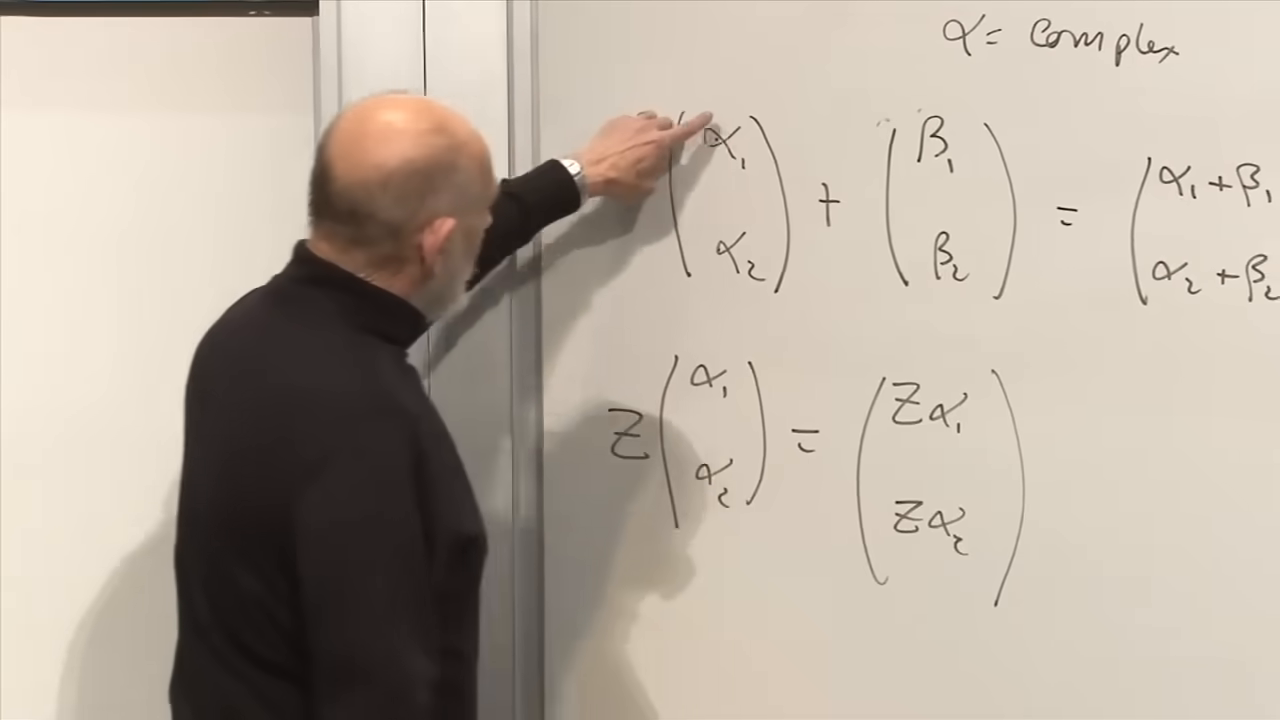
\includegraphics[width=0.88\textwidth]{lecture_01_figure_05.png}
  \caption{Покомпонентные правила сложения двух комплексных столбцов и умножения столбца на комплексный скаляр.}
  \lectureframe{01:14:28}
\end{figure}

Нулевой вектор имеет вид
\begin{equation}
  \ket{0}
  =
  \begin{pmatrix}
    0\\
    0
  \end{pmatrix},
  \qquad
  \ket{\alpha}+\ket{0}=\ket{\alpha}.
\end{equation}
Столбцы длины три образуют другое векторное пространство, и аналогично для любой фиксированной длины. Двухкомпонентный столбец нельзя складывать с трёхкомпонентным столбцом, потому что они принадлежат разным пространствам и никакое покомпонентное правило не соотносит их.

\begin{classroomqa}
\audiencequestion{Является ли вектор-столбец матрицей?}
\lecturerresponse{В общей терминологии это матрица с одним столбцом. В этом курсе слово \emph{матрица} обычно будет означать квадратную матрицу, тогда как объект с одним столбцом будет называться вектором-столбцом. Это различие терминологическое, а не разногласие относительно алгебры.}
\end{classroomqa}

\begin{classroomqa}
\audiencequestion{Имеет ли значение порядок сложения векторов?}
\lecturerresponse{Нет. Покомпонентное сложение наследует коммутативность от комплексных чисел:
\[
  \ket{\alpha}+\ket{\beta}
  =
  \ket{\beta}+\ket{\alpha}.
\]
Это одна из аксиом векторного пространства.}
\end{classroomqa}

\section{Двойственные векторы: бра и кеты}

Каждому кету \(\ket{A}\) соответствует вектор в двойственном пространстве, записываемый как \(\bra{A}\). Отображение из кета в бра аддитивно, но комплексно-сопрягает скаляры:
\begin{align}
  \ket{A}+\ket{B}
  &\longleftrightarrow
  \bra{A}+\bra{B},\\
  z\ket{A}
  &\longleftrightarrow
  z^*\bra{A}.
  \label{eq:qml1-antilinear-dual}
\end{align}
Именно это второе правило является существенной особенностью комплексного случая. Двойственный объект к скалярному кратному получается умножением на комплексно-сопряжённый скаляр.

\begin{figure}[htbp]
  \centering
  \includegraphics[width=0.86\textwidth]{lecture_01_figure_06.png}
  \caption{Соответствие между кетом и бра и его два правила: суммы переходят в суммы, а при умножении на скаляр берётся комплексное сопряжение.}
  \lectureframe{01:23:15}
\end{figure}

Для реализации с двумя компонентами,
\begin{equation}
  \ket{\alpha}
  =
  \begin{pmatrix}
    \alpha_1\\
    \alpha_2
  \end{pmatrix}
  \qquad\Longrightarrow\qquad
  \bra{\alpha}
  =
  \begin{pmatrix}
    \alpha_1^*&\alpha_2^*
  \end{pmatrix}.
  \label{eq:qml1-bra-from-ket}
\end{equation}
комплексное сопряжение осуществляет двойственное соответствие, а запись в виде строки позволяет наглядно различать два типа объектов. Равенство~\eqref{eq:qml1-bra-from-ket} также непосредственно проверяет равенство~\eqref{eq:qml1-antilinear-dual}.

\section{Скалярное произведение}

Даны \(\ket{\alpha}\) и \(\ket{\beta}\). Сочетая бра, соответствующее \(\beta\), с кетом \(\alpha\), получаем:
\begin{equation}
  \braket{\beta}{\alpha}
  =
  \begin{pmatrix}
    \beta_1^*&\beta_2^*
  \end{pmatrix}
  \begin{pmatrix}
    \alpha_1\\
    \alpha_2
  \end{pmatrix}
  =
  \beta_1^*\alpha_1+\beta_2^*\alpha_2.
  \label{eq:qml1-inner-product}
\end{equation}
Термин \emph{брэкет} буквально составлен из \emph{бра} и \emph{кет}. Это комплексный аналог обычного скалярного произведения: соответствующие компоненты перемножаются и складываются, причём для бра берётся комплексное сопряжение.

\begin{figure}[htbp]
  \centering
  \includegraphics[width=0.88\textwidth]{lecture_01_figure_07.png}
  \caption{На доске скалярное произведение \(\braket{\beta}{\alpha}\) вычисляется как \(\beta_1^*\alpha_1+\beta_2^*\alpha_2\).}
  \lectureframe{01:31:25}
\end{figure}

При перестановке векторов местами получаем
\begin{equation}
  \braket{\alpha}{\beta}
  =
  \alpha_1^*\beta_1+\alpha_2^*\beta_2
  =
  \braket{\beta}{\alpha}^{*}.
  \label{eq:qml1-conjugate-symmetry}
\end{equation}
Следовательно, порядок в общем случае важен, но различие состоит лишь в комплексном сопряжении.

\begin{classroomqa}
\audiencequestion{Можно ли определить произведение комплексных векторов, не сопрягая одну из сторон?}
\lecturerresponse{Такое билинейное выражение можно придумать, но тогда произведение вектора на самого себя не обязано быть вещественным или положительным. Эта структура не является полезной для квантовой механики. Сопряжённое, или эрмитово, скалярное произведение задаёт норму и вероятностную структуру, которые понадобятся.}
\end{classroomqa}

\subsection{Норма и положительность}

Подставим \(\beta=\alpha\) в равенство~\eqref{eq:qml1-inner-product}:
\begin{equation}
  \braket{\alpha}{\alpha}
  =
  \alpha_1^*\alpha_1+\alpha_2^*\alpha_2
  =
  |\alpha_1|^2+|\alpha_2|^2.
  \label{eq:qml1-norm-square}
\end{equation}
Это число равно своему комплексно-сопряжённому, следовательно, оно вещественно. Оно неотрицательно и обращается в нуль только для нулевого вектора. Длина определяется как
\begin{equation}
  \|\alpha\|
  =
  \sqrt{\braket{\alpha}{\alpha}}.
\end{equation}
Следовательно, комплексные компоненты дают обычную неотрицательную вещественную длину.

\begin{figure}[htbp]
  \centering
  \includegraphics[width=0.88\textwidth]{lecture_01_figure_08.png}
  \caption{На доске — скалярное произведение вектора с самим собой: \(\braket{\alpha}{\alpha}=|\alpha_1|^2+|\alpha_2|^2\), квадрат нормы.}
  \lectureframe{01:34:40}
\end{figure}

\section{Ортогональность и размерность}

Два вектора ортогональны, когда их скалярное произведение равно нулю:
\begin{equation}
  \braket{\beta}{\alpha}=0.
  \label{eq:qml1-orthogonality}
\end{equation}
Сопряжённая симметрия делает это отношение независимым от порядка:
\begin{equation}
  \braket{\beta}{\alpha}=0
  \quad\Longrightarrow\quad
  \braket{\alpha}{\beta}
  =
  \braket{\beta}{\alpha}^{*}
  =0.
\end{equation}

В двухкомпонентном пространстве простейшая ортогональная пара такова:
\begin{equation}
  \ket{e_1}
  =
  \begin{pmatrix}
    1\\
    0
  \end{pmatrix},
  \qquad
  \ket{e_2}
  =
  \begin{pmatrix}
    0\\
    1
  \end{pmatrix},
  \qquad
  \braket{e_1}{e_2}=0.
  \label{eq:qml1-standard-basis}
\end{equation}

\begin{figure}[htbp]
  \centering
  \includegraphics[width=0.88\textwidth]{lecture_01_figure_09.png}
  \caption{На доске строятся стандартные ортогональные столбцы \((1,0)^{\mathsf T}\) и \((0,1)^{\mathsf T}\).}
  \lectureframe{01:39:50}
\end{figure}

Размерность можно охарактеризовать как наибольшее число взаимно ортогональных ненулевых векторов. В двумерном пространстве таких векторов может быть два, но третьего быть не может. Чтобы увидеть это явно, пусть
\begin{equation}
  \ket{v}
  =
  \begin{pmatrix}
    v_1\\
    v_2
  \end{pmatrix}
\end{equation}
ортогонален обоим векторам из равенства~\eqref{eq:qml1-standard-basis}. Тогда
\begin{equation}
  \braket{e_1}{v}=v_1=0,
  \qquad
  \braket{e_2}{v}=v_2=0,
\end{equation}
следовательно, \(\ket{v}=\ket{0}\). Третьего ненулевого вектора, ортогонального им обоим, не существует.

\begin{classroomqa}
\audiencequestion{Разве нулевой вектор не ортогонален любому вектору, давая ещё один?}
\lecturerresponse{Да, поэтому в определении и должно говориться о \emph{ненулевых} взаимно ортогональных векторах. Нулевой вектор не задаёт независимого направления и исключается при подсчёте размерности.}
\end{classroomqa}

\begin{remark}
В представлении столбцами размерность равна числу компонент. Определение через ортогональность более абстрактно и не зависит от того, выбраны ли уже координаты.
\end{remark}

\section{Дополнительные вопросы у доски}

\begin{classroomqa}
\audiencequestion{Применима ли та же структура к векторному пространству функций?}
\lecturerresponse{Да. Функцию можно рассматривать как столбец с непрерывно индексированным семейством компонент \(\psi(x)\). Сложение и умножение на скаляр определяются поточечно. Соответствующее скалярное произведение станет интегралом, а не конечной суммой; эта конструкция будет развита позже.}
\end{classroomqa}

\begin{classroomqa}
\audiencequestion{Дает ли умножение кета на бра матрицу?}
\lecturerresponse{Да. Скалярное произведение \(\bra{\beta}\ket{\alpha}\) свёртывает строку со столбцом и даёт число. Если поменять порядок и взять \(\ket{\alpha}\bra{\beta}\), получится внешнее произведение, квадратная матрица. И скалярное, и внешнее произведения окажутся важными.}
\end{classroomqa}

\begin{classroomqa}
\audiencequestion{Действительно ли измерение воздействует на кубит, а не просто выявляет его?}
\lecturerresponse{Да. Первое измерение вдоль новой оси подготавливает новое состояние, поэтому повторение этого измерения подтверждает ответ, тогда как возвращение к старой оси снова восстанавливает неопределённость. Это неизбежное возмущение отличает квантовый эксперимент от идеализированного классического измерения, которое, по крайней мере в принципе, можно сделать сколь угодно мягким.}
\end{classroomqa}

\section{Две половины построения}

Теперь у нас есть две половины, которые ещё не соединены. Экспериментальная половина утверждает:
\begin{enumerate}
  \item идеальное измерение кубита имеет только исходы \(\pm1\);
  \item немедленное повторение того же измерения подтверждает результат;
  \item изменение оси детектора изменяет состояние, подготовленное измерением;
  \item для подготовленного ансамбля анализатор, наклонённый на \(\theta\), имеет среднее значение \(\cos\theta\).
\end{enumerate}
Математическая половина утверждает:
\begin{enumerate}
  \item квантовые состояния будут представляться векторами, а не классическими точками;
  \item соответствующие векторы образуют комплексное векторное пространство;
  \item кетам соответствуют двойственные бра, а при комплексном умножении на скаляр бра ведут себя антилинейно;
  \item эрмитово скалярное произведение определяет длину, ортогональность и размерность.
\end{enumerate}

Следующая задача — связать эти две половины. Двумерное комплексное пространство состояний кубита должно воспроизвести повторяемость, случайность и зависящую от угла статистику эксперимента с анализатором. Именно в этой связи, а не в какой-либо скрытой классической картине, и начинается квантовая механика.
